\section{The renewal law on the engine}\label{sec:validation}

\begin{figure*}[t]\centering
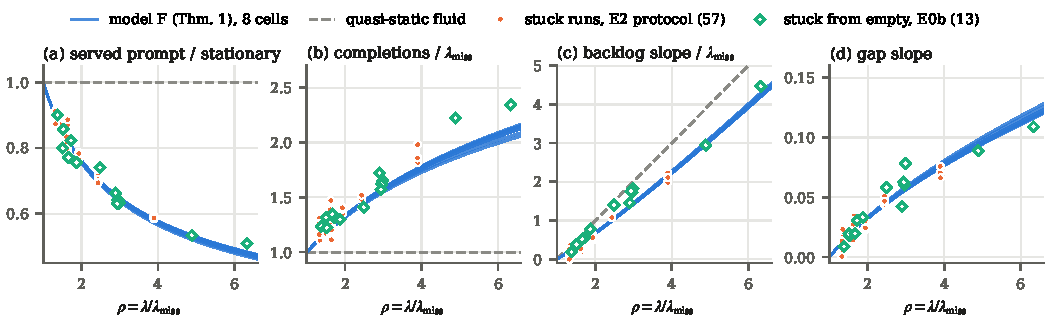
\includegraphics[width=\textwidth]{figs/fig_trap_universality.pdf}
\caption{Theorem~\ref{thm:trap} against every stuck run, as a function of the load $\rho=\lambda/\lmiss$. Points: the 57 stuck
runs of the E2 protocol (orange) and the 13 runs that lost the good state from empty (E0b, hollow). Lines: model~F for each of
the eight cells; they nearly coincide, as Corollary~\ref{cor:trapinv} predicts. No parameter is fitted to any trap
measurement. (a)~Mean prompt of the turns served, over the stationary mean: the tilted turn mix. (b)~Session completion rate
over $\lmiss$: the youth premium, above 1. (c)~Backlog growth over $\lmiss$. (d)~Growth rate of the gap between a session's
turns, $\gamma=z-1$. Dashed: the quasi-static fluid read literally in congestion (stationary composition, completion at
$\lmiss$, growth at $\rho-1$). Retrospective: the theory was derived after these runs were read.}\label{fig:trapuniv}
\end{figure*}

\begin{table}[t]
\centering\footnotesize
\caption{Theorem~\ref{thm:trap} against every stuck run of the E2 protocol (follow-up hit fraction below 0.2 over
$[5700,8700)$\,s), ranges over seeds (vLLM: registered and exploratory runs, which share plans). $\rho=\lambda/\lmiss$ with the
model's $\lmiss$. $\bar L$: mean prompt of the turns served, measured, against the tilted-mix prediction (stationary mean about
10{,}500 tokens). Gap slope: trend of the median gap between a session's turns, against $\gamma=z-1$. $D$: session completion
rate in units of $\lref$. Backlog: slope as a fraction of $\lambda-\lref$, against $\alpha/(\lambda-\lmiss)$. Retrospective; no
parameter fitted to any trap measurement; vLLM, the H200 and Llama take one speed factor fitted to their all-miss token rate.
Full table, E0b runs and pool sweep: Appendix~\ref{app:trapdata}.}\label{tab:trap}
\setlength{\tabcolsep}{1.6pt}
\resizebox{\columnwidth}{!}{%
\begin{tabular}{@{}l c c c c c@{}}
\toprule
cell, rate & $\rho$ & $\bar L$ meas.\ / pred. & gap slope / $\gamma$ & $D/\lref$ / pred. & backlog / pred.\\
\midrule
300k 1.35 & 1.34 & 9125--9556 / 9324 & .004--.020 / .013 & 1.13--1.28 / 1.13 & .14--.89 / .63\\
300k 1.65 & 1.64 & 8417--8830 / 8606 & .015--.027 / .023 & 1.25--1.35 / 1.23 & .59--.78 / .65\\
native 2.5 & 2.44 & 7264--7484 / 7374 & .044--.051 / .045 & 1.44--1.56 / 1.49 & .74--.79 / .69\\
native 4.0 & 3.90 & 6127--6213 / 6115 & .066--.076 / .081 & 1.87--2.03 / 1.81 & .68--.76 / .74\\
vLLM 1.35 & 1.32 & 9097--9547 / 9393 & .000--.016 / .012 & 1.18--1.28 / 1.14 & .00--.74 / .63\\
vLLM 1.65 & 1.62 & 8104--8778 / 8676 & .013--.028 / .022 & 1.30--1.42 / 1.24 & .41--.80 / .65\\
H200 1.5 & 1.45 & 9015--9177 / 9062 & .015--.022 / .017 & 1.20--1.27 / 1.20 & .49--.78 / .64\\
H200 2.0 & 1.93 & 8058--8230 / 8082 & .023--.031 / .032 & 1.40--1.45 / 1.36 & .51--.66 / .66\\
Llama 1.35 & 1.33 & 9075--9512 / 9356 & .003--.016 / .013 & 1.22--1.33 / 1.14 & .00--.75 / .64\\
Llama 1.65 & 1.63 & 8459--8757 / 8631 & .013--.021 / .023 & 1.34--1.49 / 1.23 & .29--.63 / .66\\
\bottomrule
\end{tabular}}
\end{table}

We test model~F on every trapped run we have, in eight cells: SGLang with the 300k pool (FCFS with and without its
waiting-prefix refresh, the BASIN, SHED and TOOLSLOW runs, and stock LPM past its 128-request fallback), SGLang's native pool,
vLLM, the H200 at 300k and 600k, Llama-3.1-8B, and the 150k and 600k pools. Each cell's costs $c_k$ come from the cost model
fitted to server-log iteration timings; vLLM, the H200 and Llama take one speed factor fitted to their own all-miss token rate.
No parameter is fitted to any trap measurement.

\paragraph{Retrospective check.} The theory was derived after these runs had been read, so this check is retrospective, not
blind. Over the 57 stuck runs of the E2 protocol (20 cell and rate groups; Table~\ref{tab:trap}, Fig.~\ref{fig:trapuniv}):
\begin{itemize}[leftmargin=*,nosep]
\item \emph{Composition.} The mean prompt of the turns served matches the tilted mix $\pi^z$ to within $-6.6$\% and $+7.7$\%,
and to within 3\% in 50 of the 57 runs. The trapped engine serves turns 10--42\% shorter than the stationary mix, and the
Perron root says by how much.
\item \emph{Gap growth.} The gap between a session's turns grows linearly in time; measured over predicted slope, the ratio has
median 0.98 (mean 0.94).
\item \emph{Youth premium.} Every stuck run completes sessions above $\lref$, at 1.10--2.40~$\lref$, and on average 1.055
times $D$ (0.90--1.21), consistent with congested engines that compute prompt tokens 1--12\% faster than the 32-session
reference behind $\lmiss$ (Appendix~\ref{app:proofs}).
\item \emph{Backlog.} The backlog grows at 0.63 of $\lambda-\lref$ on average, where model~F gives $\alpha/(\lambda-\lmiss)$ of
0.63--0.74 at these loads, not the 1.0 of the quasi-static equation.
\end{itemize}
The same laws hold for the 13 runs that lost the good state from empty, at $\rho=1.4$ to 6.3 (composition within $-5.7$\% and
$+6.6$\%; gap-slope ratio 0.62--1.30, mean 0.98), on the pool sweep and on the H200 (Appendix~\ref{app:trapdata}). Self-similarity
(Theorem~\ref{thm:trap}(d)) is visible where samples are large and censoring is small: on the H200 at 600k the sojourn of
sessions of similar length grows with their arrival time at 0.86--1.19 of the predicted slope (descriptive;
Appendix~\ref{app:trapdata}). The earlier heuristic round-robin layer of our model already reproduced the backlog slope at 300k
numerically (0.63--0.64); Theorem~\ref{thm:trap} gives the law exactly, in closed form, for every cell.

\paragraph{The registered slope rule, explained post hoc.} Our registered trap rule calls a BURST run trapped only if its
backlog slope exceeds $0.5(\lambda-\lref)$ (\S\ref{sec:evidence}). At 1.35~$\lref$ Theorem~\ref{thm:trap}(c) puts the true
slope at about $0.63(\lambda-\lmiss)$, only about 25\% above that line. The client plans are common random numbers, and seed~1's plan delivers
5.8--8.9\% fewer arrivals than nominal over the window at 1.35~$\lref$ in every cell; 8 of the 9 below-threshold runs are seed~1.
The plug-in $\lambda_{\mathrm{window}}(\text{plan})-D$, computable from the plan before any run, falls on the measured side of the
threshold for 27 of the 30 independent plans of the registered protocols, against 23 for always predicting ``trapped''. Two of
the three exceptions lie within $10^{-4}$\,/s of the threshold; the third is Llama at 1.35~$\lref$, seed~0, the registered
failure. This account is post hoc and changes no registered verdict, but it says that the indeterminate seed-1 runs are traps
whose growth the plan's arrival dip suppressed.

\paragraph{Persistence and the trigger.} No trapped FCFS run left the trap on its own. Over 50 trapped FCFS runs (49 after a
burst, one after the tool slowdown), about 100 trapped hours (99--103\,h, depending on where the trap is taken to start), no
300\,s window after the trap formed reached a follow-up hit fraction of 0.5; the highest was 0.16. A one-sided 95\% bound on a
run's probability of escaping within its observed span (at least 6100\,s) is therefore 5.8\%. Stock LPM, which leaves
request-level FCFS while its queue is short, escaped in 4 of its 9 trapped runs, and 1 of the 16 from-empty collapses (150k pool,
1.30~$\lref$, seed~0) recovered within its 3000\,s run. In 16 stuck runs (the 600k H200 paired test, BASIN bursts of 50--100
sessions, SHED's 600\,s stop and the trapped TOOLSLOW run) every trigger session had left the system 558--6246\,s before the end,
and the 727--15{,}453 turns completed after that had no hit in 15 runs (4 hits among 5{,}937 turns in the TOOLSLOW run): the trap
outlives its trigger, as Lu et al.\ also observed on hardware~\citep{lu2026cachetrap}. In the 24 registered 200-session runs on
the A100 we cannot say so: 3--30 burst sessions were still present at the end (at most 4.1\% of the sessions present). These
counts are post hoc; an independent recomputation confirmed them, with the corrections included here
(Appendix~\ref{app:dataonly}).

\paragraph{Blind tests.} The predictions of Theorem~\ref{thm:trap} for runs that did not yet exist were frozen under tag
\texttt{icml-trap-pred} (commit \texttt{6b47a6c}, pushed to the private origin at about 00:25 CST on 2026-11-05), with scoring
rules S1--S5 declared beforehand: per-run composition within $\pm8$\% (pooled $\pm5$\%), pooled gap slope within $[0.6,1.4]\gamma$,
completion above $\lref$ in every trapped run at realized load $\ge1.1\lref$ (pooled within $\pm15$\% of $D$), pooled backlog
slope within $\pm35$\% of $\alpha$, and the per-seed plug-in for the slope rule (\fpath{notes/PREDICTIONS_icml_trap.md}). The
tolerances were set after seeing the committed runs; the runs they score did not exist at the push.
\begin{itemize}[leftmargin=*,nosep]
\item \emph{TOOLSLOW-W} (registered): no burst; every tool call that starts in $[1200,3000)$\,s takes 30\,s longer, at
1.35~$\lref$, seeds 0--2, paired with the committed NOBURST runs. Its trapped runs, if any, are scored by S1--S5.
\pending{TOOLSLOW-W outcome per seed and the S1--S5 scores of its trapped runs (lead's PAPER\_INPUT).}
\item \emph{CUT} (a blind test of Corollary~\ref{cor:trapthr}): a burst at 1.65~$\lref$, then from 2400\,s arrivals cut to
1.15~$\lref$, inside $(\lmiss,D(\lambda))$ where the corollary says the trap persists although the cut rate is below the trapped
throughput, or to 0.85~$\lref$, below $\lmiss$, where it drains, but only over a busy period that $1/(1-\rho')$ stretches.
\pending{CUT predictions (tag \texttt{icml-cut-pred}) and outcomes.}
\end{itemize}

\paragraph{The arrival stop, retrodicted.} In the registered SHED test (\S\ref{sec:control}) arrivals stopped at 1800\,s,
600\,s after a burst at 1.35~$\lref$. In model~F the fluid backlog then falls to the onset $n_b=32.7$ after 2{,}020\,s and the
queue empties after 3{,}180\,s, the busy period $V_{\mathrm{tot}}(1800)$ of Theorem~\ref{thm:trap}(a) with $\lambda=0$. On the
engine, a 600\,s stop left both runs stuck, and in both 3600\,s runs hits returned 2300--2600\,s into the stop (the first
300\,s window with follow-up hit fraction of at least 0.5 began at 4100\,s; post hoc). The quasi-static model's frozen minimum
stop was 1{,}795\,s, early by about a quarter. Model~F's numbers are a retrodiction, computed after the SHED runs had ended, and
the test does not discriminate: any drain time between 600 and 3600\,s fits its two stop lengths.
